\documentclass[tikz]{standalone}

\usepackage[utf8]{inputenc}
\usepackage[T1]{fontenc}
\usepackage{lmodern}
\usepackage{uarial}
\renewcommand\familydefault{\sfdefault}
\usepackage{xcolor}
% Grattan colors
\definecolor{Orange}{HTML}{F68B33}
\definecolor{OrangeBackground}{RGB}{254,240,222}  % for boxes
\definecolor{Color1}{RGB}{255,224,127}
\definecolor{Color2}{RGB}{255,195,90}
\definecolor{Color3}{RGB}{246,139,51}
\definecolor{Color4}{RGB}{212,88,42}
\definecolor{Color5}{RGB}{160,34,38}
\definecolor{Color6}{RGB}{98,18,20}
\definecolor{theGrey}{HTML}{6A737B}
\definecolor{AuthorPage}{RGB}{160,34,38}
\definecolor{AuthorGrey}{RGB}{174,174,174}
 
\tikzset{add reference/.style={insert path={%
    coordinate [pos=0,xshift=-0.5\pgflinewidth,yshift=-0.5\pgflinewidth] (#1 south west)
    coordinate [pos=1,xshift=0.5\pgflinewidth,yshift=0.5\pgflinewidth]   (#1 north east)
    coordinate [pos=.5] (#1 center)                       
    (#1 south west |- #1 north east)     coordinate (#1 north west)
    (#1 center     |- #1 north east)     coordinate (#1 north)
    (#1 center     |- #1 south west)     coordinate (#1 south)
    (#1 south west -| #1 north east)     coordinate (#1 south east)
    (#1 center     -| #1 south west)     coordinate (#1 west)
    (#1 center     -| #1 north east)     coordinate (#1 east)  
}}}
\usetikzlibrary{shapes,arrows}
\tikzstyle{block} = [rectangle, draw, 
    text width=4em, text centered, rounded corners, minimum height=4em]
    
    \tikzstyle{line} = [draw, -latex']

\begin{document}
 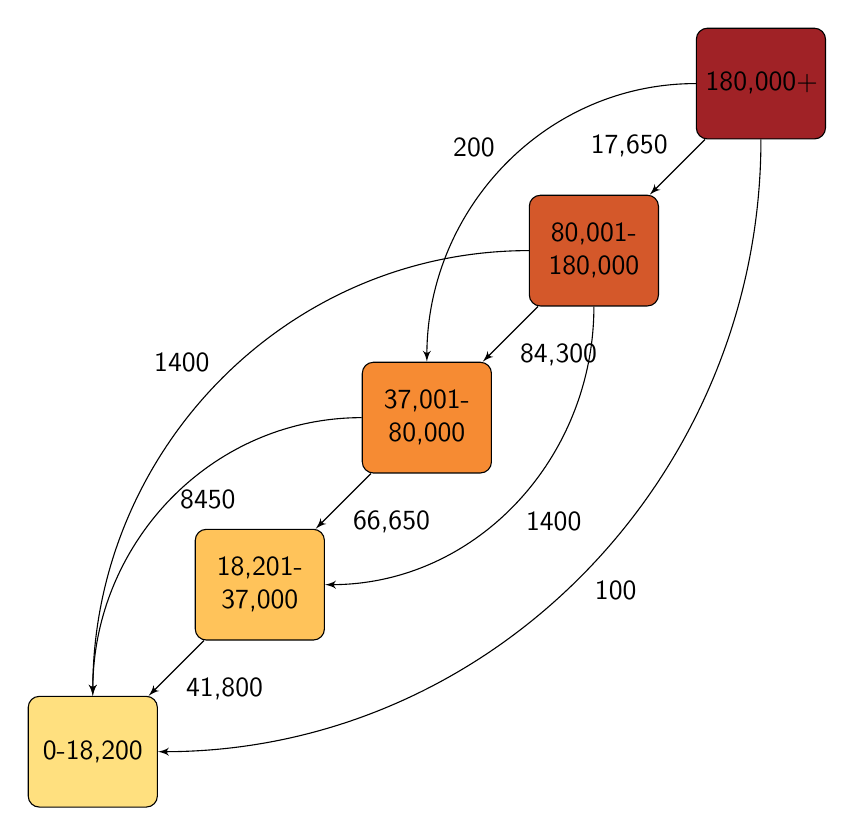
\begin{tikzpicture}[node distance = 3cm, auto]
  \node [block, fill=Color1] (Under) {0-18,200};
  \node [block, fill=Color2, above right of = Under] (Low) {18,201-37,000};
  \node [block, fill=Color3, above right of = Low] (Middle) {37,001-80,000};
  \node [block, fill=Color4, above right of = Middle] (Upper) {80,001-180,000};
  \node [block, fill=Color5, above right of = Upper] (High) {180,000+};
  %
  \path [line] (Low) --node{41,800} (Under);
  %
  \path [line] (Middle) to[out = 180, in = 90, anchor=west]node{8450} (Under);
  \path [line] (Middle) --node{66,650} (Low);
  %
  \path [line, fill=white] (Upper) --node{84,300} (Middle);
  \path [line] (Upper) to[out = 180, in = 90, anchor=south east]node{1400} (Under);
  \path [line] (Upper) to[out = -90, in = 0] node{1400} (Low);
  %
  \path [line] (High) --node[anchor=south east]{17,650} (Upper);
  \path [line] (High) to[out = 180, in = 90, anchor=south east]node{200} (Middle);
  \path [line] (High) to[out = -90, in = 0]node{100} (Under);
 \end{tikzpicture}

\end{document}
